\documentclass[english]{beamer}
\listfiles

\usepackage{babel}
\usepackage[utf8]{inputenc}
\usepackage[T1]{fontenc}
\usepackage{bm}
\usepackage{graphicx}
\usepackage{siunitx}
\usepackage{booktabs}
\usepackage{xfrac}
\usepackage{algorithmic}
\usepackage{enumerate}
\usepackage{xmpincl}
\includexmp{CC_Attribution_3.0_Unported}
\usepackage{ccicons}

\mode<presentation>
{
  \usetheme{aausidebar}
  \setbeamercovered{invisible}
}

\title{Modern \LaTeX{} Usage}

\author[Thomas Arildsen]
{
  Thomas Arildsen\\
  \href{mailto:tha@es.aau.dk}{{\ttfamily tha@es.aau.dk}}\\
  \ccby
}

\institute[TPS, Dept. of Electronic Systems, Aalborg University]
{ TPS\\
  Dept. of Electronic Systems\\
  Aalborg University}

\date{}

\subject{LaTeX}

\pgfdeclareimage[height=1cm]{university-logo}{figures/aau_segl_en}
\logo{\pgfuseimage{university-logo}}

\begin{document}

\begin{frame}[plain]
  \titlepage
\end{frame}

\begin{frame}{Licensing and Availability}
  \begin{block}{}
    Modern LaTeX Usage by Thomas Arildsen is licensed under a
    \href{http://creativecommons.org/licenses/by/3.0/}{Creative
      Commons Attribution 3.0 Unported License}.
    \begin{center}
      \ccby
    \end{center}
  \end{block}
  \begin{block}{}
    Source available from
    \href{https://github.com/ThomasA/modernLaTeX}{GitHub}.
  \end{block}
  \begin{block}{}
    PDF slides available from
    \href{http://dx.doi.org/10.6084/m9.figshare.763250}{figshare}
    (\mbox{DOI: 10.6084/m9.figshare.763250}).
  \end{block}
\end{frame}

\begin{frame}{Appetizer}
  An attempt to provide some information on best-practice use of LaTeX
  for typesetting scientific material for reports, articles,
  presentations, theses etc.

  This is not a complete introduction to \LaTeX. I assume basic
  knowledge of using \LaTeX{} in advance. For those interested in an
  introduction, please see:
  \href{ftp://ftp.dante.de/tex-archive/info/lshort/english/lshort.pdf}{The
    Not So Short Introduction to \LaTeX}.

  Some of this advice comes from the document
  ``\href{ftp://ftp.dante.de/tex-archive/info/l2tabu/english/l2tabuen.pdf}{l2tabu}'',
  which I strongly encourage you to read as well.
\end{frame}

\begin{frame}{Agenda}
  \tableofcontents
  % You might wish to add the option [pausesections]
\end{frame}

%\section{Background}

\section{\LaTeX{} Distributions}

% TexLive, MikTeX, MacTeX

\begin{frame}{\insertsection}{TeX Live}
  TeX Live is a very comprehensive distribution containing more or
  less everything \TeX.
  \begin{itemize}
  \item Cross-platform (Unix/Linux, MacOS, Windows) -- comes will all
    binaries compiled for these platforms.
  \item Has built-in package manager to update and install additional
    packages.
  \item Available here: \url{http://texlive.org}
  \end{itemize}
\end{frame}

\begin{frame}{\insertsection}{MacTeX}
  MacTeX is derived from TeX Live but customized for MacOS.
  \begin{itemize}
  \item MacOS only.
  \item Basically a TeX Live with some extras for MacOS and everything
    configured for MacOS out-of-the-box.
  \item Available here: \url{http://www.tug.org/mactex/}
  \end{itemize}
\end{frame}

\begin{frame}{\insertsection}{MiKTeX}
  MiKTeX is somewhat like TeX Live a very comprehensive distribution
  that gives you more or less anything you might need.
  \begin{itemize}
  \item Windows only.
  \item Has a very clever package manager that will even retrieve
    missing package on-the-fly while compiling.
  \item Available here: \url{http://miktex.org/}
  \end{itemize}
\end{frame}

\section{(La)TeX flavours and workflows}

% Flavours:
% TeX: Knuth's original (1978)
% LaTeX: Leslie Lamport (started early 1980's); 2.09, 2e, 3 (future,
% in dev. since early 1990's).
% pdfTeX/pdfLaTeX: Direct compilation to PDF, font handling
% improvements, e.g. native TrueType and Type 1 font embedding, direct
% access to PDF features sucg as hyperlinks, TOC etc.
% LuaTeX/LuaLaTeX: (2007) Started from pdfTeX + Lua scripting and native
% opentype font support + unicode, multi-directional typesetting,
% system fonts.
% XeTeX/XeLaTeX: (2004) Advanced font support with system fonts and
% special features such as special glyphs, ligatures etc. Native unicode.

\begin{frame}{\insertsection}{\TeX}
  \TeX{} is the original typesetting system developed by Donald Knuth
  from 1978.
  \begin{itemize}
  \item Perceived by many as being genius.
  \item Famous for superb typesetting capabilities.
  \item Currently maintained and latest release from 2008.
  \end{itemize}
\end{frame}

\begin{frame}{\insertsection}{\LaTeX}
  \LaTeX{} is a macro overlay for \TeX{} that defines a higher-level
  ``language'' on top of \TeX{} making it much easier to format
  documents.
  \begin{itemize}
  \item Developed by Leslie Lamport from the early 1980's.
  \item The current version is \LaTeX{} $2_\varepsilon$.
  \item The newer \LaTeX{} 3 has been under way since the early 1990's.
  \item Extensive collection of packages for doing more or less
    anything in \LaTeX.
  \end{itemize}
\end{frame}

\begin{frame}{\insertsection}{pdfTeX/pdfLaTeX}
  pdfTeX is an extension of \TeX{} with more modern features. pdfLaTeX
  is its \LaTeX{} counterpart.
  \begin{itemize}
  \item Direct compilation to PDF.
  \item Font handling improvements, e.g. native TrueType and Type 1
    font embedding.
  \item Direct access to PDF features such as hyperlinks, TOC etc.
  \item \emph{Breaks compatibility with EPS graphics} (no
    pstricks/psfrag).
  \end{itemize}
\end{frame}

\begin{frame}{\insertsection}{LuaTeX/LuaLaTeX}
  LuaTeX is another (newer) extension of \TeX.
  \begin{itemize}
  \item Originates from pdfTeX. AFAIK official successor of pdfTex.
  \item Incorporates scripting in the Lua language.
  \item Native opentype font support.
  \item Native unicode.
  \item Native multi-directional typesetting.
  \item \emph{Can use system fonts}.
  \end{itemize}
\end{frame}

\begin{frame}{\insertsection}{XeTeX/XeLaTeX}
  XeTeX is yet another extension of \TeX{} in a sligthly different
  direction than LuaTeX.
  \begin{itemize}
  \item Advanced font support with system fonts and special features
    such as special glyphs, ligatures etc.
  \item Native unicode.
  \end{itemize}
\end{frame}

% Workflows:
% latex -> dvi -> ps -> pdf
% latex -> dvi -> pdf
% latex -> pdf (pdflatex)

\begin{frame}{\insertsection}{\LaTeX{} $\rightarrow$ DVI $\rightarrow$
    PostScript $\rightarrow$ PDF}
  The classic workflow in LaTeX: \LaTeX{} $\rightarrow$ DVI
  $\rightarrow$ PostScript $\rightarrow$ PDF.
  \begin{itemize}
  \item Uses the '\texttt{latex}' executable to generate a DVI file.
  \item The DVI file is converted to PostScript using '\texttt{dvips}'.
  \item If you want PDF, you can further convert the PostScript to PDF
    using, e.g., '\texttt{ps2pdf}' or Adobe Distiller.
  \end{itemize}
  Originally from the days before anyone thought of PDF.
\end{frame}

\begin{frame}{\insertsection}{DVI $\rightarrow$ PDF}
  More direct path to PDF: \LaTeX{} $\rightarrow$ DVI $\rightarrow$ PDF.
  \begin{itemize}
  \item Uses the '\texttt{latex}' executable to generate a DVI file.
  \item The DVI file is converted to PDF using '\texttt{dvipdf}'.
  \end{itemize}
  Simpler approach if you want PDF but for some reason must go through
  DVI (e.g., pstricks or psfrag).
\end{frame}

\begin{frame}{\insertsection}{\LaTeX{} $\rightarrow$ PDF}
  The modern approach if you really just want a PDF: \LaTeX{}
  $\rightarrow$ PDF.
  \begin{itemize}
  \item Uses the '\texttt{pdflatex}' executable to generate a PDF file.
  \end{itemize}
  It is my impression that many long-time \LaTeX{} users still don't
  know this option.
\end{frame}

%\section{Fonts and formatting}

\section{Fonts}

%\subsection{Using fonts}

% Font packages with math support

\begin{frame}{\insertsection}{Choosing different fonts}
  Handling fonts can be a nightmare in \LaTeX. You typically have two
  options:'
  \begin{itemize}
  \item Stick to \LaTeX's default ``Computer Modern'' font - a
    Times-like font.
  \item Become an expert on \LaTeX's font handling to customize the
    use of fonts in your document.
  \end{itemize}
  I recommend a third, intermediate solution: use fonts that are
  available as packages in your system.
\end{frame}

\begin{frame}{\insertsection}{Font packages}
  These packages encapsulate all the hard-core mechanics for setting
  up the font and come with the necessary files (somewhere, don't
  worry about them).

  A good place to start:
  \begin{itemize}
  \item List of fonts with math support and examples shown:
    \href{http://www.tug.dk/FontCatalogue/mathfonts.html}{http://www.tug.dk/FontCatalogue/mathfonts.html}.
  \end{itemize}
\end{frame}

%\subsection{Text style selection}

\begin{frame}[fragile]{\insertsection}{Font shape}
  People are often seen using obsolete font commands from earlier
  versions of LaTeX, such as \verb|{\bf }|, \verb|{\it }| etc. The
  correct current use of font selection should be:
  \begin{table}
    \centering
    \begin{tabular}{lcc}
      Shape & Small piece of text & Current environment\\
      \midrule
      \textbf{Bold}          & \verb|\textbf{...}| & \verb|\bfseries| \\ 
      \emph{Emphasized}      & \verb|\emph{...}|   & \verb|\em|       \\ 
      \textit{Italic}        & \verb|\textit{...}| & \verb|\itshape|  \\ 
      \textmd{Medium weight} & \verb|\textmd{...}| & \verb|\mdseries| \\ 
      \textrm{Roman}         & \verb|\textrm{...}| & \verb|\rmfamily| \\ 
      \textsc{Small caps}    & \verb|\textsc{...}| & \verb|\scshape|  \\ 
      \textsf{Sans serif}    & \verb|\textsf{...}| & \verb|\sffamily| \\ 
      \textsl{Slanted}       & \verb|\textsl{...}| & \verb|\slshape|  \\ 
      \texttt{Typewriter}    & \verb|\texttt{...}| & \verb|\ttfamily| \\ 
      \textup{Upright}       & \verb|\textup{...}| & \verb|\upshape| 
    \end{tabular}
  \end{table}
\end{frame}
% Selection commands inside text, exemplify no-gos
% Make a point about double newlines, \noindent etc.

\section{Text Encoding}

\begin{frame}[fragile]{\insertsection}{Dealing with ``special''
    characters}
  Traditionally, in \LaTeX{} you will deal with uncommon characters by
  using certain commands, for example:
\begin{verbatim}
\"u \'e \`e \ae{} \o{} \aa{}
\end{verbatim}
  Result: \"u \'e \`e \ae{} \o{} \aa{}

  Instead, we can simply choose a text encoding that supports the
  needed characters, e.g., UTF-8, using the \textbf{inputenc} package:
\begin{verbatim}
\usepackage[utf8]{inputenc}
\end{verbatim}
  ---
\begin{verbatim}
ü é è æ ø å
\end{verbatim}
  Result: ü é è æ ø å
\end{frame}

\section{Document Formatting}

%\subsection{Margins and Line Spacing}

% geometry, setspace

\begin{frame}{\insertsection}{Margins}
  There is a low-level mechanism to control margins etc. in \LaTeX{} by
  setting various ``lengths''.
  \begin{figure}
    \centering
    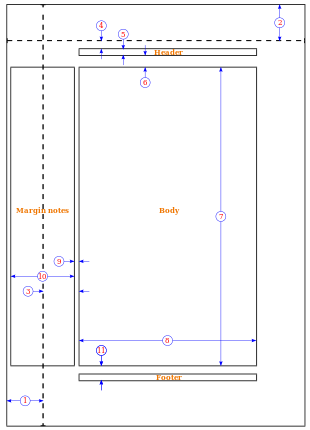
\includegraphics[height=5cm]{Latex_layout.png}
    \caption{Figure by
      \href{http://commons.wikimedia.org/wiki/File:Latex_layout.svg}{Alessio
        Damato} -- CC BY-SA 3.0}
  \end{figure}
\end{frame}

\begin{frame}[fragile]{\insertsection}{Margins}
  \LaTeX{} page layout can be a real pain to configure.
  \begin{itemize}
  \item Nice solution: the \textbf{geometry} package.
  \end{itemize}
\begin{verbatim}
\usepackage[margin=2cm]{geometry}
\end{verbatim}
  Just a simple example of \SI{2}{\centi\meter} margin on all
  sides. Far more details can be specified.
\end{frame}

\begin{frame}[fragile]{\insertsection}{Line space}
  \LaTeX{} line spacing can be set at various abstraction levels and
  can be difficult to set consistently for all elements of the
  document.
  \begin{itemize}
  \item Again a nice solution: the \textbf{setspace} package.
  \end{itemize}
\begin{verbatim}
\usepackage{setspace}

\singlespacing
\onehalfspacing
\doublespacing
\setstretch{<factor>} % for custom spacing
\end{verbatim}
  It also provides environments for locally setting the spacing.
\end{frame}

%\subsection{Various Document Classes}

\begin{frame}[allowframebreaks]{\insertsection}
  \LaTeX{} comes with a selection of standard document classes for
  various purposes, such as: {\bfseries article, report, book}. These
  are fine for most purposes.

  If you are curious about other document classes, the following are a
  few examples of high-quality document classes:
  \begin{description}
  \item[KOMA Script] Provides the three main classes {\bfseries
      scrartcl, scrreprt, scrbook}. Customizable. The page layout of
    these classes is said to be more ``European/A4''-friendly than
    \LaTeX's standard counterparts.
  \item[Memoir] Also very customizable class. Book-like structure,
    allowing parts and chapters, but can be used for articles and
    reports as well. Good for theses.
  \item[IEEEtran] The standard class for most (all?) of IEEE's
    journals. This is a high-quality article class that you could use
    for other documents of your own as well as papers submitted to
    IEEE.
  \item[Tufte-latex] Provides the classes \textbf{tufte-book} and
    \textbf{tufte-handout} by Edward Tufte. A quite different but
    interesting layout. Check it out if you are a bit adventurous.
  \end{description}
\end{frame}
% KOMA-Script (is said to have more European/A4-friendly layout)
% Memoir
% IEEEtran
% tufte-latex (for the very inspired...)

%\section{Mathematics, Numbers and Data}

\section{Mathematics}

\begin{frame}[allowframebreaks,fragile]{\insertsection}{Packages for
    typesetting mathematics}
  \LaTeX{} was ``born'' being excellent for typesetting mathematical
  symbols, formulae etc. There are however a few useful packages to
  make your life even easier:
  \begin{description}
  \item[amsmath] This package, along with \textbf{amsfonts} and
    \textbf{amssymb} provide a host of useful math features. Most
    notable are its several equation environment building blocks such
    as {\bfseries align, aligned, alignat, split, multline, gather,
      gathered} as well as environments for building matrices and
    definitions for different cases.
  \item[xfrac] Provides the command \verb|\sfrac| which prints
    fractions like this $\sfrac{1}{2}$, which may look better in text
    than the usual $\frac{1}{2}$.
  \item[bm] People probably often encounter the problem of making
    greek-letter variables appear bold, for example to signify
    matrices or vector. This package provides the solution, the
    command \verb|\bm|:
\begin{verbatim}
$\bm{\epsilon} \bm{\Phi}$
  vs.
$\mathbf{\epsilon} \mathbf{\Phi}$
\end{verbatim}
    ---

    $\bm{\epsilon} \bm{\Phi}$ vs. $\mathbf{\epsilon} \mathbf{\Phi}$
  \end{description}
\end{frame}

\begin{frame}[fragile]{\insertsection}{Other math tips \& tricks}
  \begin{itemize}
  \item Never use the \textbf{eqnarray} environment. Use
    \textbf{amsmath}'s \textbf{align} or similar instead.
    
    For background, see
    \href{http://tug.org/pracjourn/2006-4/madsen/madsen.pdf}{tug.org/pracjourn/2006-4/madsen/madsen.pdf}.
  \item A useful ``trick'' is to define variable names etc. for your
    equations as commands, for example:
\begin{verbatim}
\newcommand{\myVector}{\mathbf x}

$\myVector = \mathbf 0$
\end{verbatim}
    ---

    \newcommand{\myExtremelyImportantVector}{\mathbf x}
    $\myExtremelyImportantVector = \mathbf 0$

    This makes it easy to replace the variable name to, say, $\mathbf
    y$ instead when your supervisor asks you to, all 237 places in the
    document. Simply edit your command definition!
  \end{itemize}
\end{frame}

% amsmath etc.
% Never eqnarray
% defining variable names as commands
% xfrac
% bm

\section{Numbers and Units}

% siunitx (also tables)
\begin{frame}[fragile]{\insertsection}{Pretty-printing}
  The package \textbf{siunitx} provides consistent printing of numbers
  with units.
  \begin{itemize}
  \item As the name suggests, it handles all SI units, but also other
    units such as bits, bytes etc.
\begin{verbatim}
\SI{40}{\meter\per\second}
\end{verbatim}
    ---
    
    \SI{40}{\meter\per\second}
  \item Also handles consistent printing of numbers with
    customizable precision and many other features.
\begin{verbatim}
\num[scientific-notation = true,
     round-mode = figures,
     round-precision = 5]{5345.2528592868725}
\end{verbatim}
    ---
    
    \num[scientific-notation = true, round-mode = figures,
    round-precision = 5]{5345.2528592868725}
  \end{itemize}
\end{frame}

\section{Data}

\begin{frame}{\insertsection}{Displaying data from files}
  What if you have a comma separated file of data that you want to
  display? Copy-and-paste it into your source?
  \begin{itemize}
  \item The package \textbf{datatool} can actually read data from
    comma-separated or similar text-based files.
  \item Lets you build tables from the loaded values.
  \item Can even plot the data using the auxiliary program
    \textbf{gnuplot}.
  \end{itemize}
\end{frame}

%\section{Various Floats and Listings}

\section{Floating Material}

% centering vs. center environment

\begin{frame}[fragile]{\insertsection}{Centering floats}
  It is often seen that people use the \textbf{center} environment
  inside floats (for example \textbf{figure, table}) to center the
  content.
  \begin{itemize}
  \item This may cause unwanted extra vertical space around your
    figure, table etc.
  \item Simple fix: use \verb|\centering| instead:
\begin{verbatim}
\begin{figure}[h]
  \centering
  ...
\end{figure}
\end{verbatim}
  \end{itemize}
\end{frame}

% subfig, not subfigure

\begin{frame}[fragile]{\insertsection}{Sub-figures, -tables etc.}
  Sometimes you want to collect several figures into one major figure
  environment (``Fig. 1a, 1b and 1c'', for example).
  \begin{itemize}
  \item This can be achieved using the \textbf{subfig} package and its
    \verb|\subfloat| command that wraps the sub-figure, -table
    etc. inside the containing \textbf{figure, table}
    etc. environment.
  \item Use \textbf{subfig} and not \textbf{subfigure}. The latter is
    outdated.
  \end{itemize}
\end{frame}

% wrapfig (not floating but something similar)

\begin{frame}{\insertsection}{Wrapping text around a figure}
  \LaTeX{} places floats so that they occupy the entire horizontal
  space around them, with no text alongside them. This improves
  readability and is usually preferred.

  If you really want to flow text around a figure, this can be done:
  \begin{description}
  \item[wrapfig] This package lets text wrap around a figure. The
    figure no longer floats, but text will be placed alongside it.
  \item[flowfram] This package lets you do very advanced stuff with
    text flowing around shapes that can be defined in a drawing
    program.
  \end{description}
\end{frame}

% Placing graphics HERE - the mistake that graphics do not have to be
% a float, placing a float HERE, not worrying about it.

\section{Graphics}

% graphicx, not graphics, epsfig etc.
% psfrag
\begin{frame}{\insertsection}{Displaying from files}
  \LaTeX{} can display graphics from various file formats. This can be
  done using the packages \textbf{graphics} and \textbf{graphicx}.
  \begin{itemize}
  \item Both packages come from the same ``family'', \textbf{graphics}
    just has a simpler interface than its extended cousin
    \textbf{graphicx}.
  \item Use these packages instead of \textbf{epsf.sty, psfig.sty,
      epsfig.sty}; these are outdated.
  \end{itemize}
\end{frame}

% PGF/TiKZ + externalize graphics
% matlab2tikz
% jpgfdraw
\begin{frame}{\insertsection}{Making \LaTeX{} draw graphics}
  You can make \LaTeX{} generate graphics according to a script.
  \begin{itemize}
  \item \LaTeX{} has some built-in drawing commands that I will not
    get into here.
  \item PSTricks is a package that enables very advanced
    drawings. Unfortunately, this is based on PostScript and does not
    work with pdfLaTeX (PDF).
  \item PGF/TiKZ is a package (or packages: \textbf{pgf} and
    \textbf{tikz} -- they are two complementary layers of macro
    languages) that also enables very advanced drawing.

    This works both for DVI $\rightarrow$ PS and PDF. HIGHLY RECOMMENDED.
  \item PGF/TiKZ can use a feature to ``externalize'' graphics,
    meaning that new drawings are generated on first compilation and
    subsequently loaded from EPS/PDF files.

    Improves speed and provides stand-alone graphics files.
  \end{itemize}
\end{frame}

\begin{frame}{\insertsection}{TiKZ, pgfplots and Matlab}
  PGF/TiKZ have a companion package \textbf{pgfplots} that can be used
  to plot graphs of data very nicely.
  \begin{itemize}
  \item \textbf{pgfplots} can be used on its own to set up plots.
  \item Another option is to use it for plotting figures from Matlab.

    The matlab script ``matlab2tikz'' can be used to convert Matlab
    figures to \textbf{pgfplots} code that can be rendered in \LaTeX{}
    using PGF/TiKZ.

    Found here: \url{http://www.mathworks.com/matlabcentral/fileexchange/22022}
  \item Huge advantage: all text and numbers in the plots are
    generated by \LaTeX{} and will automatically match the style of
    the rest of your document.
  \end{itemize}
\end{frame}

%\section{Tables}

% tables: longtable (page breaking), tabularx (automatic column
% widths), booktabs, colortbl

\section{Listings}

% algorithm + algorithmicx (pseudo-code)
% lisings (source code)
% Customizing enumerate

\begin{frame}[fragile,allowframebreaks]{\insertsection}{Algorithms and
    pseudocode}
  We often need to list an algorithm or a piece of pseudo-code in a
  document.
  \begin{itemize}
  \item A useful package for this purpose is \textbf{algorithmic}.
  \item Provides the environment \textbf{algorithmic} for typesetting
    the actual code listing.
\begin{verbatim}
\begin{algorithmic}
  \FOR{$i=0$ to $10$}
  \STATE carry out some processing
  \ENDFOR
\end{algorithmic}
\end{verbatim}
    ---
    \begin{algorithmic}
      \FOR{$i=0$ to $10$} \STATE carry out some processing
      \ENDFOR
    \end{algorithmic}
  \item The \textbf{algorithmic} environment just produces the code
    text block.
  \item To create a floating environment (like a table or figure),
    wrap it in the \textbf{algorithm} environment.
\begin{verbatim}
\begin{algorithm}
  \caption{Some algorithm.}
  \begin{algorithmic}
    \FOR{$i=0$ to $10$}
    \STATE carry out some processing
    \ENDFOR
  \end{algorithmic}
\end{algorithm}
\end{verbatim}
    ---

    (Cannot show the \textbf{algorithm} float in Beamer\ldots)
  \end{itemize}
\end{frame}

\begin{frame}{\insertsection}{Source code}
  We sometimes need to list actual source code, e.g., Python, C,
  Matlab etc., as opposed to pseudo-code.
  \begin{itemize}
  \item A useful package for this purpose is \textbf{listings}.
  \item Can display and markup source code from a large selection of
    languages, including C, Python, Matlab, TeX, LaTeX\ldots
  \item Can list code pasted in the document or read code from an
    external file.
  \item Highly custumizable, can display line numbers, can display
    excerpts of code.
  \end{itemize}
\end{frame}

\begin{frame}[fragile]{\insertsection}{Enumerate}
  This is not really related to source code, but this is nice to know
  as well.
  \begin{itemize}
  \item You can customize enumerate environments using the
    \textbf{enumerate} package.
  \item It lets you easily and intuitively change the numbering of
    items. For example:
\begin{verbatim}
\begin{enumerate}[2.I]
\item One
\item Two
\item Three
\end{enumerate}
\end{verbatim}
    ---

    \begin{enumerate}[2.I]
    \item One
    \item Two
    \item Three
    \end{enumerate}
  \end{itemize}
\end{frame}

%\section{Referencing and Indexing}

\section{Easy References}

\begin{frame}[fragile]{\insertsection}{Cleveref}
  Do you ever get tired of keeping track of writing
  ``\verb|Fig.~\ref{...}|'', ``\verb|Eq.~(\ref{...})|'' etc. when
  cross-referencing in your documents?
  \begin{itemize}
  \item The package \textbf{cleveref} can handle this automatically.
  \item Simply reference using \verb|\cref{...}| in stead of \verb|\ref{...}|.
  \item Cleveref will automatically figure out what you are
    referencing and add ``Figure'', ``Table'' etc. accordingly.
  \item Highly customizable in great detail in terms of what to call
    things; ``Figure'', ``figure'', or ``Fig.'' etc.
  \item References can be converted to plain text if a journal does
    not support \textbf{cleveref}, using the 'poorman' option.
  \end{itemize}
\end{frame}
% cleveref + 'poorman'

%\section{Glossaries and Acronyms}

% glossaries

\section{Bibliographies}

% Classic BibTeX, extend with bibtex8 for unicode support.
% Biblatex + biber

\begin{frame}{\insertsection}
  \LaTeX{} traditionally uses BibTeX to generate bibliographies in
  documents.
  \begin{itemize}
  \item BibTeX is an old lady and does not dance with unicode text for example.
  \item The straight-forward fix is to use the ``bibtex8'' program
    instead of ``bibtex''.

    Allows using bibliography files encoded in for example UTF-8 as
    mentioned earlier so it can handle special characters such as: æ,
    ø, å, ð etc. typed directly in the bibliography file.
  \end{itemize}
\end{frame}

\begin{frame}{\insertsection}
  There is a new bibliography package in town!
  \begin{itemize}
  \item Biblatex is a complete re-design of bibliographies for \LaTeX.
  \item Very customizable.
  \item Very advanced features (chapter-wise bibliographies,
    localization\ldots)
  \item Natively handles modern input encodings such as unicode.
  \item Works together with the backend program ``Biber'' that sorts
    the bibliography, instead of ``bibtex''.
  \item Drawback: not supported by IEEE yet.
  \end{itemize}
\end{frame}

%\section{Index}

% makeidx
% index/xindy

\section{Presentations and Posters}

% Beamer
% Jesper Kjær's template

\begin{frame}{\insertsection}{Beamer}
  Why use PowerPoint?
  \begin{itemize}
  \item No-one can edit your files---at least not those running
    Linux ;-)
  \item You cannot display mathematics properly.
  \end{itemize}
  Don't worry. \LaTeX{} is your friend here too.
  \begin{itemize}
  \item Using the package \textbf{beamer}, you can easily format slide
    shows directly in LaTeX.
  \item Produces PDFs which can be read by everyone, displayed anywhere.
  \item Beamer has loads of mechanisms to make content change, appear
    or disappear on slides.
  \end{itemize}
\end{frame}

\begin{frame}{\insertsection}{Suggested theme}
  This presentation was made in Beamer.
  \begin{itemize}
  \item The ``theme'' used in these slides was created by Jesper Kjær
    Nielsen from MISP.
  \item The theme is available here:
    \url{http://kom.aau.dk/~jkn/latex/latex.php}.
  \end{itemize}
\end{frame}

% baposter
% Jesper Kjær's template

\begin{frame}{\insertsection}{Poster template}
  We often need to print posters for presentations at conferences.
  \begin{itemize}
  \item One possibility is the package \textbf{baposter}.
  \item It works by letting you create ``boxes'' that you fill content into.
  \item The relative positioning of these boxes can be specified and
    their sizes are automatically taken care of.
  \item A couple of the posters in our hallway were made using this
    package with a theme created by, again, Jesper Kjær Nielsen.
  \item The theme is available here:
    \url{http://kom.aau.dk/~jkn/latex/latex.php}.
  \end{itemize}
\end{frame}

\section{PhD Theses}

\begin{frame}{\insertsection}{Recommended class}
  Some of you need to start thinking about writing your thesis soon\ldots...
  \begin{itemize}
  \item One useful class to do this is \textbf{memoir}, mentioned
    earlier (I used this for my thesis).
  \item Well-suited for large documents.
  \item Good-looking layout.
  \item Easily customizable.
  \item The previously mentioned KOMA Script bundle should also be
    very suitable.
  \end{itemize}
\end{frame}

\begin{frame}[fragile]{\insertsection}{Including papers}
  Often you will want to do your thesis as a collection of papers. You
  have all these previously formatted papers that do not fit into your
  thesis layout. What do you do about them?
  \begin{itemize}
  \item A clever solution is provided by the package \textbf{docmute}.
  \item You include documents using the  \verb|\include| command.
  \item Docmute will automatically remove the preamble of any
    documents included this way, so they will ``obey'' the formatting
    of your master document.
  \end{itemize}
\end{frame}

\begin{frame}{\insertsection}{Bibliographies}
  When including bibliographies in your thesis, each included paper
  will usually have its own bibliography.
  \begin{itemize}
  \item The previously mentioned package \textbf{biblatex} can handle
    this elegantly.
  \item Using the feature ``refsection'' or ``refsegment'',
    \textbf{biblatex} can keep track of what you reference in which
    section (or segment) and number and list these references for the
    individual sections.
  \end{itemize}
\end{frame}

% docmute
% biblatex for chapter bibliographies

\end{document}

% LocalWords:  quantizer
